%% ----------------------------------------------------------------
%% AppendixA.tex
%% ---------------------------------------------------------------- 

\chapter{First-layer filters} \label{Chapter:Feat}
\begin{figure}
\centering
\includegraphics[width=1\linewidth]{Figures/allfilters3}\\
\caption{\textit{Filters of the first layer with size three.} The $y$ axis is the depth of the network, with the upper 21 rows corresponding to the one-hot encoded amino-acids and the bottom 21 rows to the \textit{pssm} values. $x$ axis is the window size (width). Red values are positive and blue values are negative.}
\label{fig:allfilters3}
\end{figure}

\begin{figure}
	\centering
	\includegraphics[width=1\linewidth]{Figures/allfilters5}
	\caption{\textit{Filters of the first layer with size five.} The $y$ axis is the depth of the network, with the upper 21 rows corresponding to the one-hot encoded amino-acids and the bottom 21 rows to the \textit{pssm} values. $x$ axis is the window size (width). Red values are positive and blue values are negative.}
	\label{fig:allfilters5}
\end{figure}

\begin{figure}
	\centering
	\includegraphics[width=1\linewidth]{Figures/allfilters7}
	\caption{\textit{Filters of the first layer with size seven.} The $y$ axis is the depth of the network, with the upper 21 rows corresponding to the one-hot encoded amino-acids and the bottom 21 rows to the \textit{pssm} values. $x$ axis is the window size (width). Red values are positive and blue values are negative.}
	\label{fig:allfilters7}
\end{figure}

\chapter{Saliency map aggregations} \label{Chapter:App}
\begin{figure}
\centering
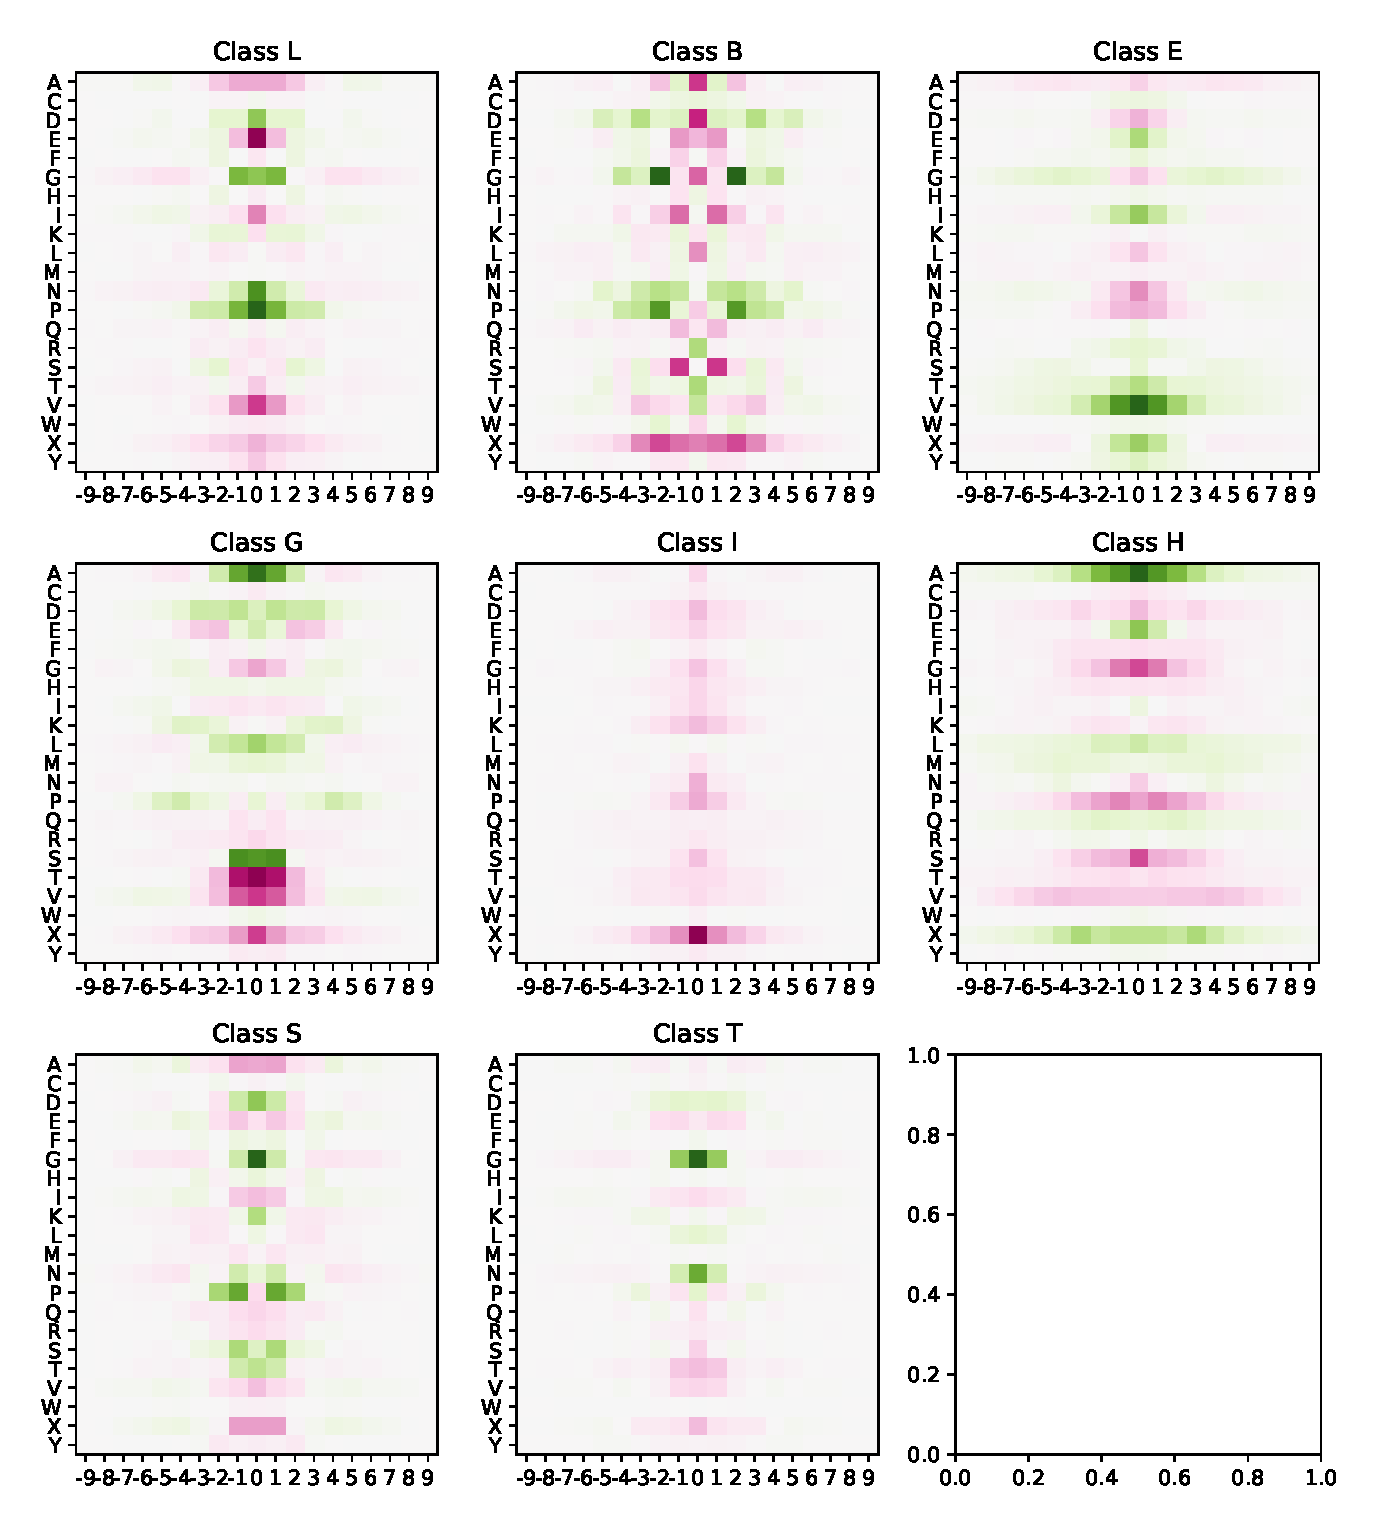
\includegraphics[width=0.85\linewidth]{Figures/class_agg_class_all}
\caption{\textit{Per-class aggregated saliency maps along the window of all classes, as discussed in Section \ref{sect:sheer}.} Only the saliency values of \textit{pssm} are shown here. Green means positive saliency values and purple means negative.}
\label{fig:class_agg_class_all}
\end{figure}

\begin{figure}
\centering
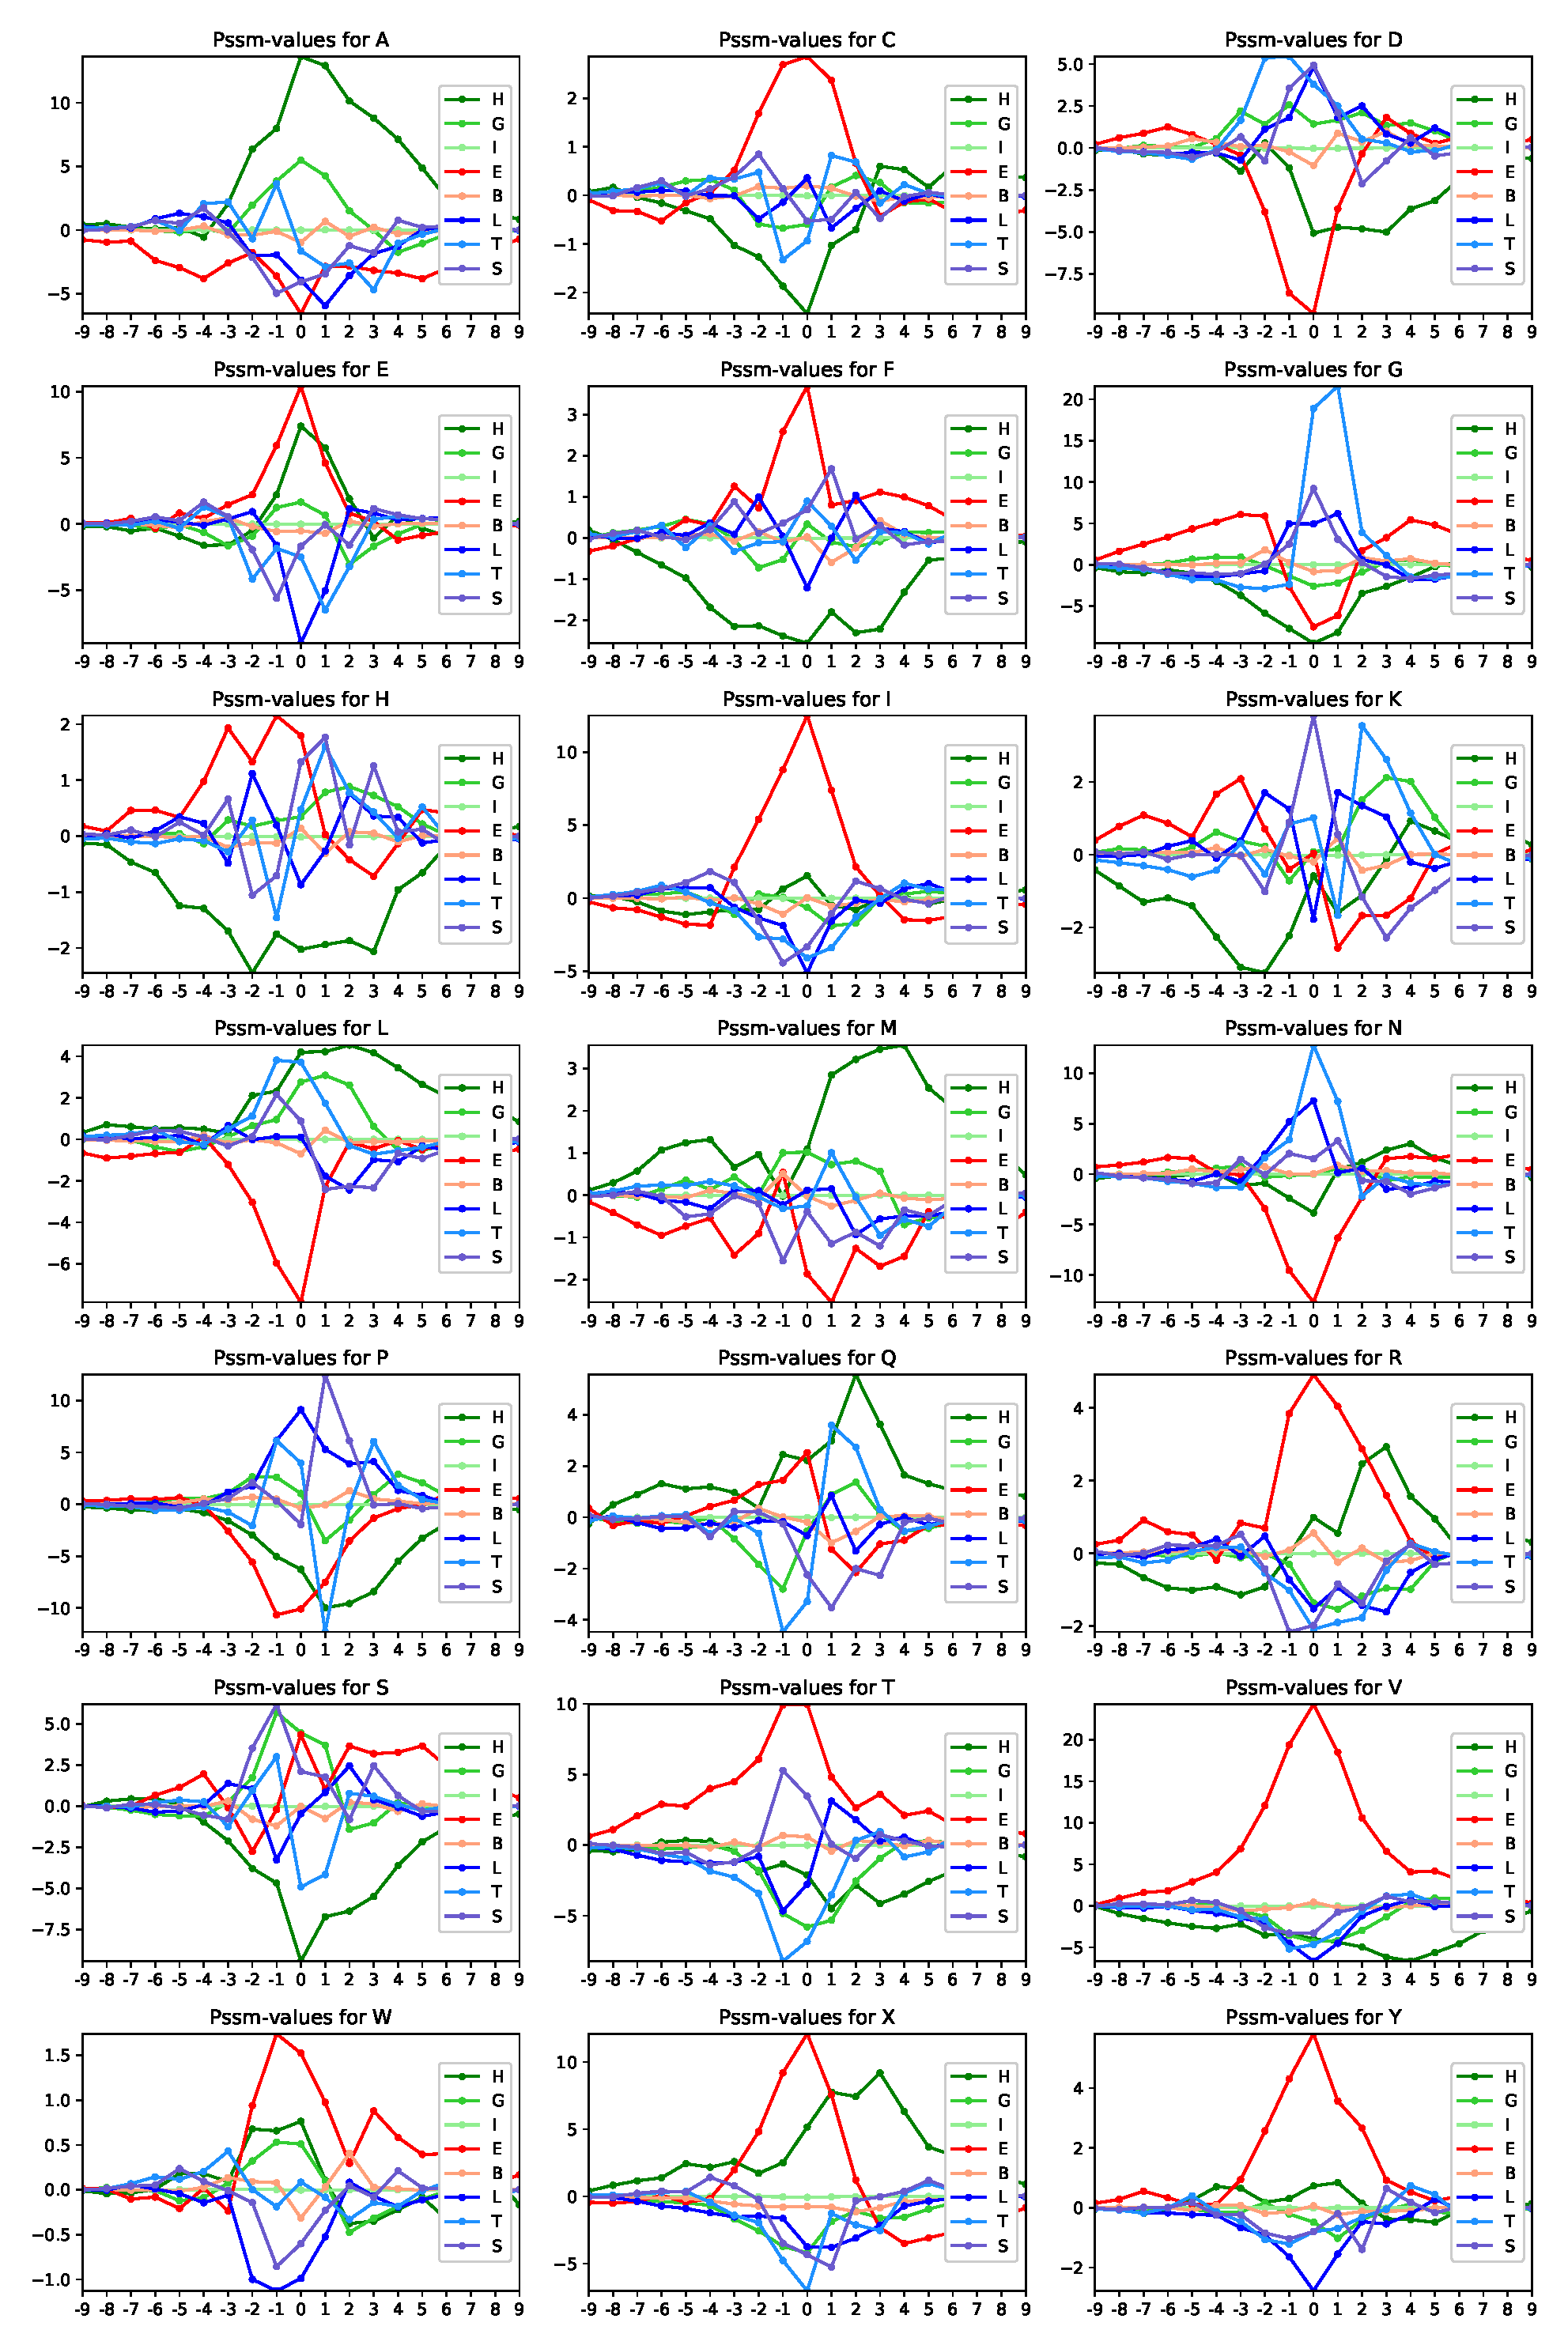
\includegraphics[width=1\linewidth]{Figures/class_agg_aa_all}
\caption{\textit{Per-class aggregated saliency map of all 21 amino-acids.} \textit{Y} axis is in 1000s. Note the changes in scale.}
\label{fig:class_agg_aa_all}
\end{figure}

\chapter{Project planning}
\begin{figure}
	\centering
	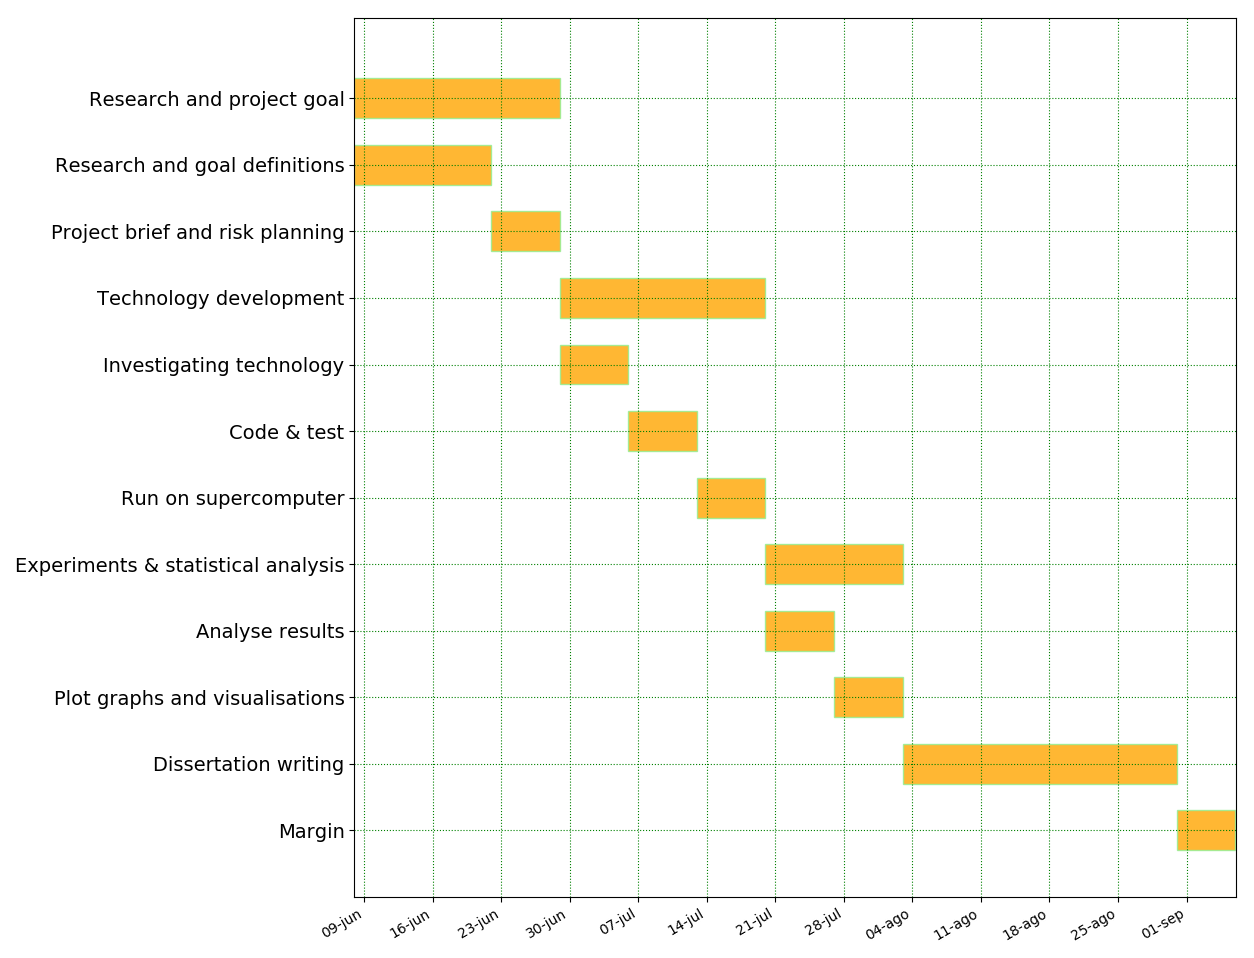
\includegraphics[width=1\linewidth]{Figures/gantt}
	\caption{\textit{Gantt chart of the project planning.} Although the time was divided into four distinct phases (\textit{Research}, \textit{Technology development}, \textit{Experiments}, and \textit{Dissertation writing}), there has been some overlapping between them.}
	\label{fig:gantt}
\end{figure}